\documentclass{article}
\usepackage[space]{ctex}
\usepackage{graphicx}
\usepackage{float}
\usepackage{hyperref}
\graphicspath{{../article_pic/}}
\begin{document}
循环神经网络按时间轴展开的时候,如下图所示:
\begin{figure}[H]
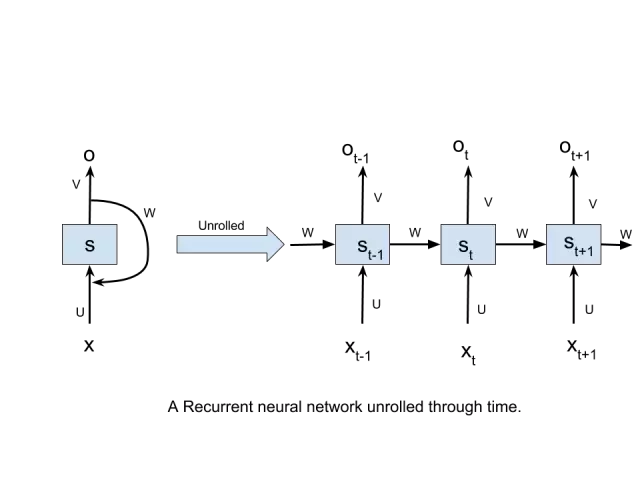
\includegraphics[scale=0.5]{rnn_unroll.png}
\end{figure}
图中:
\begin{enumerate}
\item $x_t$ 代表时间步 t 的输入;
\item $s_t$ 代表时间步 t 的隐藏状态,可看作该网络的「记忆」;
\item $o_t$ 作为时间步 t 时刻的输出;
\item U、V、W 是所有时间步共享的参数,共享的重要性在于我们的模型在每一时间步以不同的输入执行相同的任务。
\end{enumerate}
当把 RNN 展开的时候,网络可被看作每一个时间步都受上一时间步输出影响(时间步之间存在连接)的前馈网络。

两个注意事项

为了更顺利的进行实现,需要清楚两个概念的含义:
\begin{enumerate}
\item TensorFlow 中 LSTM 单元格的解释;
\item 数据输入 TensorFlow RNN 之前先格式化。
\end{enumerate}

TensorFlow 中 LSTM 单元格的解释

在 TensorFlow 中,基础的 LSTM 单元格声明为:

tf.contrib.rnn.BasicLSTMCell(num\_units)


这里,num\_units 指一个 LSTM 单元格中的单元数。num\_units 可以比作前馈神经网络中的隐藏层,前馈神经网络的隐藏层的节点数量等于每一个时间步中一个 LSTM 单元格内 LSTM 单元的 num\_units 数量。下图可以帮助直观理解:

\begin{figure}[H]
	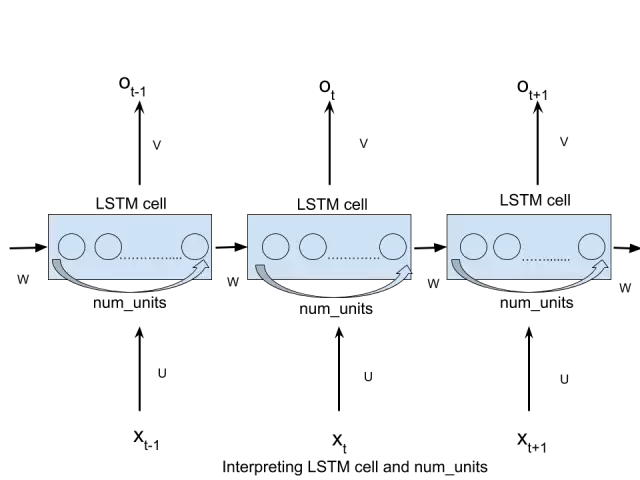
\includegraphics[scale=0.5]{lstm_unit.png}
\end{figure}
每一个 num\_units LSTM 单元都可以看作一个标准的 LSTM 单元:


以上图表来自博客(\href{http://colah.github.io/posts/2015-08-Understanding-LSTMs/}{地址}),该博客有效介绍了 LSTM 的概念。

数据输入 TensorFlow RNN 之前先格式化

在 TensorFlow 中最简单的 RNN 形式是 static\_rnn,在 TensorFlow 中定义如下:

tf.static\_rnn(cell,inputs)


虽然还有其它的注意事项,但在这里我们仅关注这两个。

inputs 引数接受形态为 [batch\_size,input\_size] 的张量列表。列表的长度为将网络展开后的时间步数,即列表中每一个元素都分别对应网络展开的时间步。比如在 MNIST 数据集中,我们有 28x28 像素的图像,每一张都可以看成拥有 28 行 28 个像素的图像。我们将网络按 28 个时间步展开,以使在每一个时间步中,可以输入一行 28 个像素(input\_size),从而经过 28 个时间步输入整张图像。给定图像的 batch\_size 值,则每一个时间步将分别收到 batch\_size 个图像。详见下图说明:
\begin{figure}[H]
	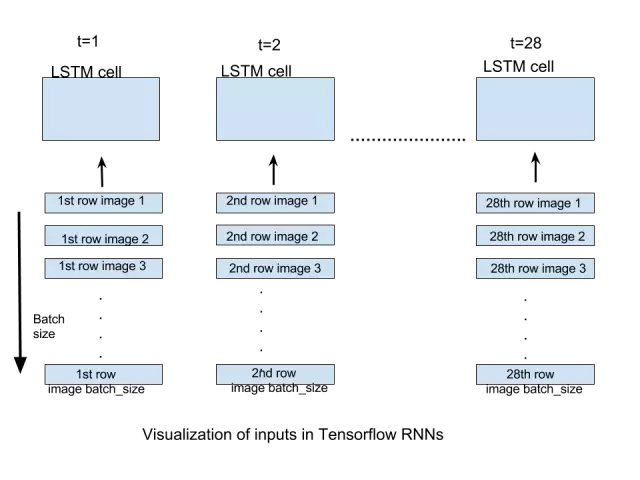
\includegraphics[scale=0.5]{tf_rnn.png}
\end{figure}
由 static\_rnn 生成的输出是一个形态为 [batch\_size,n\_hidden] 的张量列表。列表的长度为将网络展开后的时间步数,即每一个时间步输出一个张量。在这个实现中我们只需关心最后一个时间步的输出,因为一张图像的所有行都输入到 RNN,预测即将在最后一个时间步生成。
\end{document}
